\section{zadanie 1}
Zadanie polegało na implementacji algorytmów obliczających równania macierzowe

\subsection{Metoda Eliminacji Gaussa, opis algorytmu: }
Podstawowa metoda eliminacji Gaussa sprowadza się do dwóch kroków:\\
1. przekształcenia macierzy pierwotnej [ A \(\vert\) b ] do postaci trójkątnej górnej\\

\[
\begin{bmatrix}
  a_{11}^{(0)} & a_{12}^{(0)} & \cdots & a_{1n}^{(0)} & | & b_{1}^{(0)} \\
  a_{21}^{(0)} & a_{22}^{(0)} & \cdots & a_{2n}^{(0)} & | & b_{2}^{(0)}\\
  \vdots & \vdots & \ddots & \vdots & | & \vdots\\
  a_{n1}^{(0)} & a_{n2}^{(0)} & \cdots & a_{nn}^{(0)} & | & b_{n}^{(0)}
\end{bmatrix}
\]\[
\downarrow
\]\[
\begin{bmatrix}
  a_{11}^{(k)} & a_{12}^{(k)} & \cdots & a_{1n}^{(k)} & | & b_{1}^{(k)} \\
  0 & a_{22}^{(k)} & \cdots & a_{2n}^{(k)} & | & b_{2}^{(k)}\\
  \vdots & \vdots & \ddots & \vdots & | & \vdots\\
  0 & 0 & \cdots & a_{nn}^{(k)} & | & b_{n}^{(k)}
\end{bmatrix}
\]

2. rozwiązania trójkątnego układu równań
\begin{align*}
a_{11}^{(k)} x_1 + a_{12}^{(k)} x_2 + \ldots + a_{1n}^{(k)} x_n = b_{1}^{(k)}\\
a_{22}^{(k)} x_2 + \ldots + a_{2n}^{(k)} x_n = b_{1}^{(k)}\\
\vdots\\
a_{nn}^{(k)} x_n = b_{n}^{(k)}
\end{align*}

Pamiętając całą macierz w naiwmy sposób potrzebujemy \(O(n^2)\) miejsca a czasowa złożoność algorytmu wyniesie \(O(n^3)\)

\subsection{Metoda Eliminacji Gaussa, optymalizacja: }
Przez specyficzną postać macierzy podanej w zadaniu możemy zoptymalizować złożoność czasową rozwiązywania układu rówań. Ponieważ w ogólnym rozwiązaniu podczas pierwszego kroku pętla będzie wykonywała się od \textbf{k+1} do \textbf{n} możemy pominąć wszystkie zera pod przekątną i wykonać to przejście od \textbf{k+1} do \textbf{min(n, k + l + 1)} wtedy czasowa złożoność obliczeniowa tych pętli będzie w czasie O(1) zatem zostanie jedynie pętla zewnętrzna i cały algorytm wykona się w czasie liniowym.
\begin{align*}
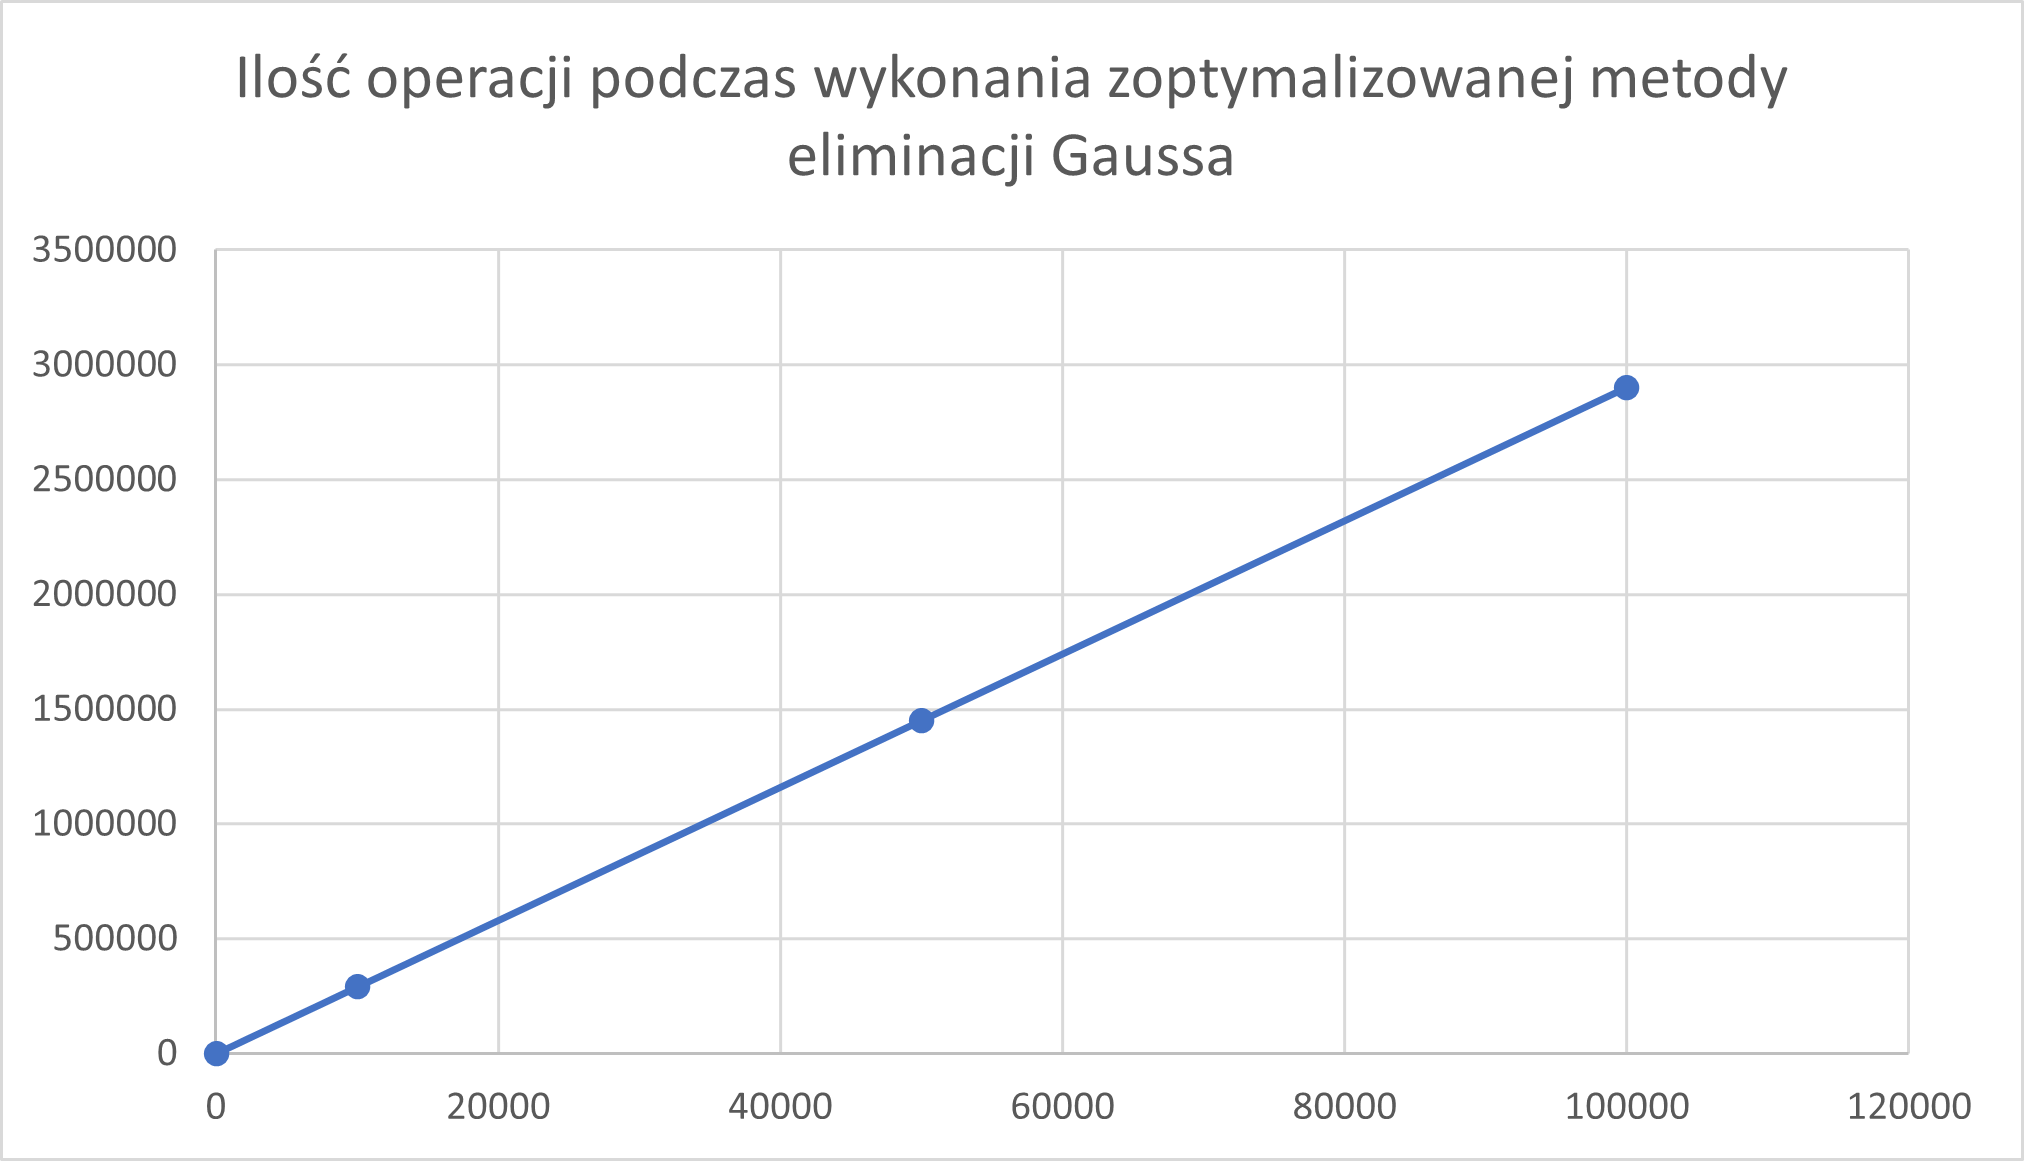
\includegraphics[width=\textwidth]{wykres.png}
\end{align*}

\subsection{Wnioski: }
Dla rozwiązywania układów równań na szczególnych macierzach warto szukać sposobów optymalizacji oraz jeśli macierze są rzadkie używać struktur danych, które przechowają dane w bardziej efektywny sposób